\documentclass[a4paper, 11pt]{article}
\usepackage[left=2cm,text={17cm, 24cm},top=3cm,left= 2cm]{geometry}
\usepackage[IL2]{fontenc}
\usepackage[czech]{babel}
\usepackage[utf8]{inputenc}
\usepackage{graphicx}
\usepackage{subcaption}
\usepackage{float}
\usepackage{url}
\providecommand{\uv}[1]{\quotedblbase #1\textquotedblleft}
\DeclareUrlCommand\url{\def\UrlLeft{<}\def\UrlRight{>} \urlstyle{tt}}

\begin{document}
\thispagestyle{empty}
\begin{center}
\Huge
\textsc{Vysoké učení technické v Brně}\\
\huge
\textsc{Fakulta informačních technologií}\\
\LARGE
\vspace{\stretch{0.382}}
Modelování a simulace - 6. Počítačové služby\\ \Huge Porovnávání SQL a JAVA přístupů do databáze
\vspace{\stretch{0.618}}
\end{center}

{
\LARGE \hfill
Vojtěch Meluzín - xmeluz04\\
\today \hfill
Matěj Mlejnek - xmlejn04}

\newpage
\thispagestyle{empty}

\tableofcontents

\newpage
\setcounter{page}{1}
\section{Úvod}
V této práci je řešen projekt do předmětu \textbf{IMS - Modelování a simulace} \cite{ims_web} vyučovaném na Fakulta informačních technologií Vysokého učení technického v Brně \cite{fit_web}. Konkrétně se jedná o zadání \textbf{6. Počítačové služby} \cite{zadani_web}.

Tato práce se věnuje problematice vyhledávacích časů nad databází, kde jsme se zaměřili na zkoumání časových rozdílů mezi SQL dotazy a načítáním do RAM paměti s následným procházením po jednotlivých řádcích. Následné vygenerované data analyzujeme a modelujeme v simlibu\cite{simlib_web, simlib_zdroj}
\subsection{Zdroje faktů}
Jako model jsme si vybrali databázi Postgresql \cite{postgresql_web}. Pro přístup do této databáze jsme zvolili naprogramování aplikace v jazyce JAVA \cite{java_web} ve verzi JDK-1.8.0\_151 \cite{java_jdk_version}, ve které jsme si naprogramovali komunikaci se serverem. Programy pro sběr dat z této komunikace běželi na virtualním stroji Ubuntu 16.04.3 LTS \cite{ubuntu_web} a samotné posílání jednotlivých dotazů bylo zautomatizované pomocí scriptu psaném v GNU Bash version 4.3.48(1)-release (x86\_64-pc-linux-gnu) \cite{bash_web}.

\subsection{Ověření funkčnosti modelu}
Validita modelu byla ověřována porovnáváním výstupních hodnot a reálných dat.

\section{Fakta}
K filtraci na straně databáze jsme použili podmínku id like PRESNOST||

Na straně javy jsme filtrovali pomocí String metody startsWith(PRESNOST)

Presnost nám udávala pocet známích číslic ze zečátku hledaného id. Například pokud bylo hledané id 9653 a přesnot 2 tak do dotazu jsme dosazovali 96. Přesnost byla maximálně 4.

\subsection{Vícenásobný běh}
\newpage
\begin{figure}[H]
\centering
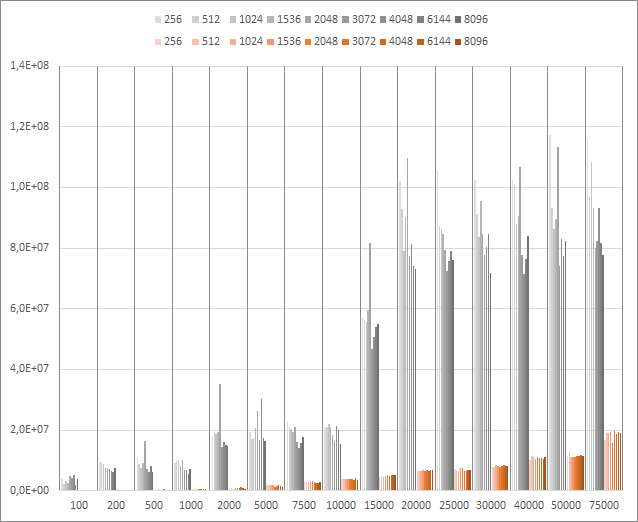
\includegraphics[width=100mm]{images/n1-100-75k.png}
\caption{LIKEE 1 - 100-75 000}
\end{figure}
\begin{figure}[H]
\centering
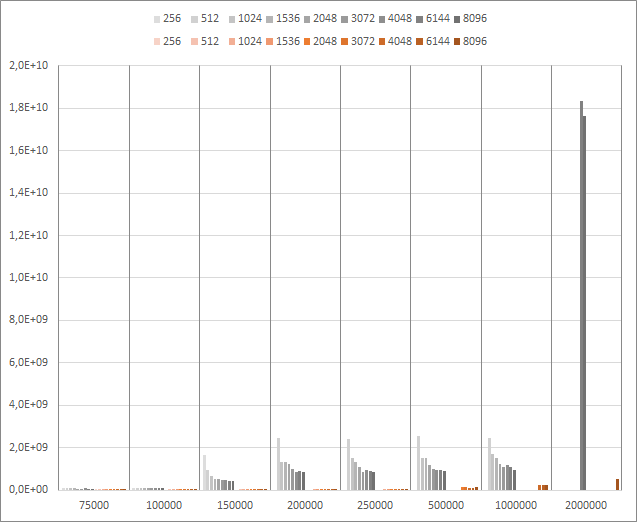
\includegraphics[width=100mm]{images/n1-75k-2kk.png}
\caption{LIKEE 1 - 75 000-2 000 000}
\end{figure}
\begin{figure}[H]
\centering
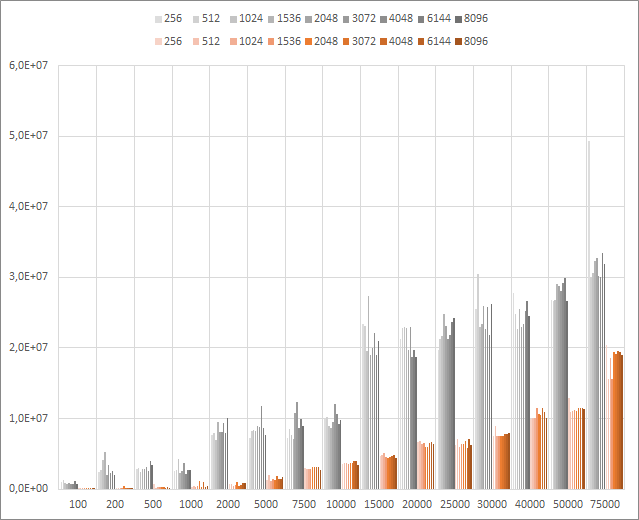
\includegraphics[width=100mm]{images/n10-100-75k.png}
\caption{LIKEE 10 - 100-75 000}
\end{figure}
\begin{figure}[H]
\centering
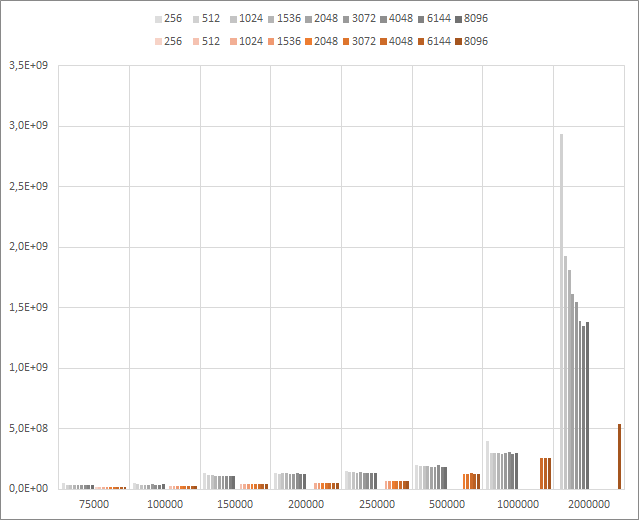
\includegraphics[width=100mm]{images/n10-75k-2kk.png}
\caption{LIKEE 10 - 75 000-2 000 000}
\end{figure}
\begin{figure}[H]
\centering
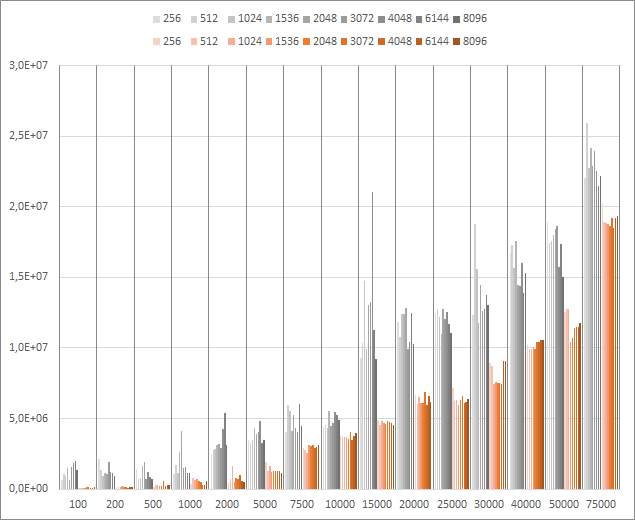
\includegraphics[width=100mm]{images/n100-100-75k.png}
\caption{LIKEE 100 - 100-75 000}
\end{figure}
\begin{figure}[H]
\centering
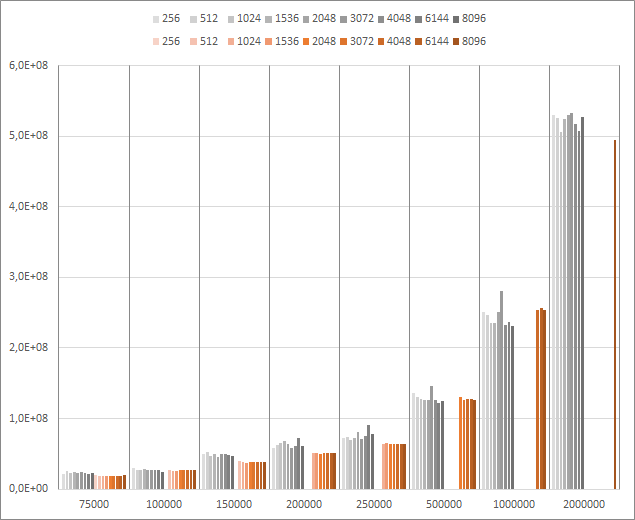
\includegraphics[width=100mm]{images/n100-75k-2kk.png}
\caption{LIKEE 100 - 75 000-2 000 000}
\end{figure}
\begin{figure}[H]
\centering
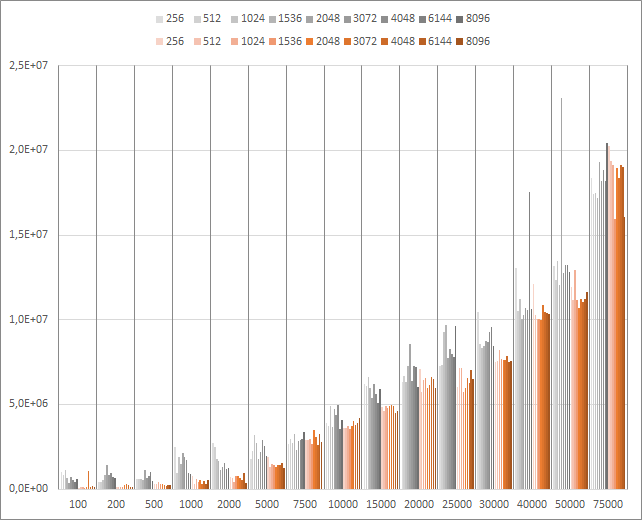
\includegraphics[width=100mm]{images/n1000-100-75k.png}
\caption{LIKEE 1000 - 100-75 000}
\end{figure}
\begin{figure}[H]
\centering
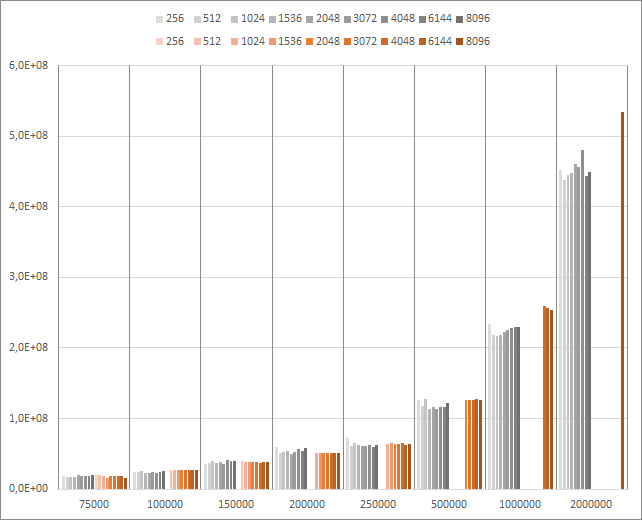
\includegraphics[width=100mm]{images/n1000-75k-2kk.png}
\caption{LIKEE 1000 - 75 000-2 000 000}
\end{figure}






\section{Koncepce modelu}

\subsection{Petriho sít}
\begin{figure}[H]
\centering
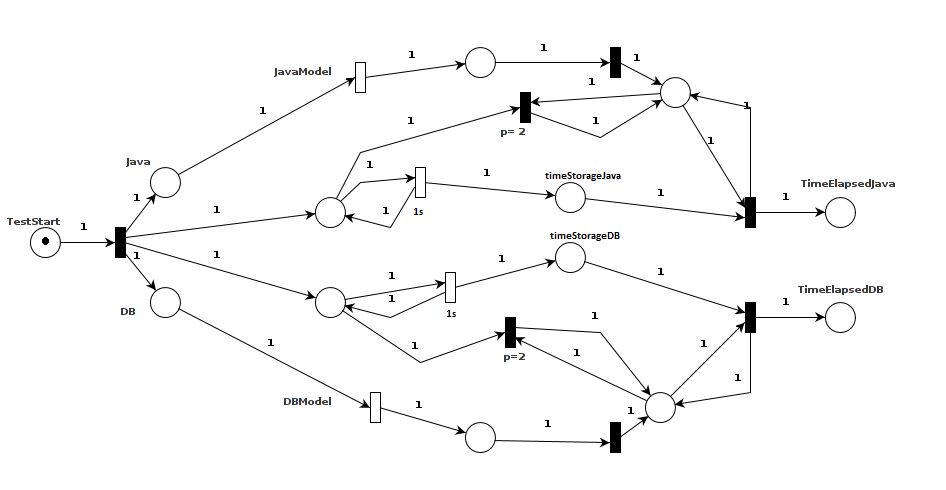
\includegraphics[width=150mm]{images/Petri-net-1.png}
\caption{Petriho sít}
\end{figure}

\begin{figure}[H]
\centering
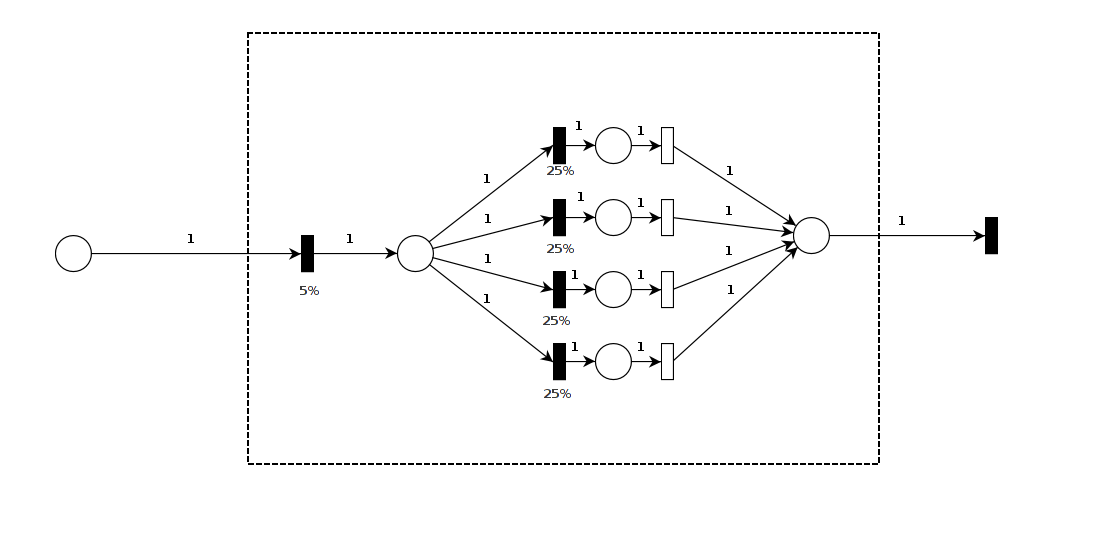
\includegraphics[width=150mm]{images/Petri-net-2.png}
\caption{DBModel a JavaModel}
\end{figure}


\section{Závěr}
Po porovnání doby vykonání 10 000 náhodných dotazů v simulačním prostředí jsme zjistili, že pokud budeme potřebovat jen tabulky, které se dají celé pojmout pamětí v JAVA, tak se nám vždy vyplatí filtrace za pomocí JAVA.

256 MB
Db: 71292.617176
Java: 14097.718977

512 MB
Db: 12415280.999453
Java: 12154.622090

1024 MB
Db: 4052740.756615
Java: 11117.939846

2048 MB
Db: 64080.730505
Java: 10295.285151

4048 MB
Db: 52820.119157
Java: 10218.761830

8096 MB
Db: 47365.118296
Java: 9890.339874

\pagebreak
\newpage
\bibliographystyle{czechiso}
\def\refname{Literatura}
\bibliography{proj4}

\end{document}